\chapter{蒙特卡洛数值模拟与机制检验}\label{ch:simulations}

\section{模拟实验规格与算法设计}\label{sec:sim_spec}

前两章分别在单代静态点估计、跨期平稳基准以及多期运筹设计下推导了解析方差结构。为了在复杂的非平衡状态与小样本离散条件下核验理论解析式的紧致性，并深入剖析时间序列动态更新过程中的预测误差演化机制，本章构建大规模蒙特卡洛随机模拟实验系统。

\subsection{算法环境与负二项离散生成机制}
所有数值算法均基于 Python 3.10 环境自主编写，核心随机数生成与离散分布计算依赖 \texttt{scipy.stats} 与 \texttt{numpy} 科学计算库。在算法实现中：
\begin{itemize}
    \item 负二项分布统一采用紧凑参数化形式 $\NB(r, p)$。由第二章定理~\ref{thm:closure}，在给定条件期望均值 $\mu = \rho n R_t$、风险集规模 $n$ 及过度离散参数 $k$ 下，形状参数映射为 $r = nk$，成功概率映射为 $p^* = \frac{k}{k + \rho R_t}$；
    \item 离散累积尾部概率与分位数临界值通过对数尺度生存函数 \texttt{stats.nbinom.sf(c - 1, r, p)} 计算，以避免浮点数下溢；
    \item 蒙特卡洛独立重复试验规模：图 1 单代静态验证采用 50,000 次蒙特卡洛模拟（固定随机种子 20260923）；图 2 假设检验功效采用每参数网格 30,000 次模拟（随机种子 20260924）；图 3 时间序列动态更新过程每规模网格生成 150 条独立疫情时序轨迹，每条轨迹包含 30 代连续传播。
\end{itemize}

\section{命题 5：超临界增长检测的精确检验与离散功效锯齿}\label{sec:prop5_power}

本节针对推断目标二（疫情爆发早期预警检验），研究如何在小样本与超传播条件下建立一致最优检验。

\subsection{单调似然比（MLR）一阶对数差分严格为正证明}
公共卫生早期预警的核心任务是检验疫情是否失控，对应单侧假设检验问题：
\begin{equation}
H_0: R_t \le 1 \quad \text{vs} \quad H_1: R_t > 1. \label{eq:hypothesis_testing}
\end{equation}

\begin{proposition}[\textbf{命题 5：超临界增长精确检验与离散功效}]\label{prop:prop5}
设已知 $(n, \rho, k)$，观测病例数为 $C_t$。
\begin{enumerate}[label=(\roman*)]
    \item 分布族关于充分统计量 $C_t$ 具有严格单调似然比（MLR）性质，上尾拒绝域：
    \begin{equation}
    \mathcal{W}_\alpha = \{C_t \ge c_\alpha\}, \quad c_\alpha = \min\big\{ c \in \mathbb{N} : \Pr_{R_t=1}(C_t \ge c) \le \alpha \big\},
    \end{equation}
    在显著性水平 $\alpha$ 下构成复合原假设 $H_0$ 下的一致最优（UMP）水平控制检验；
    \item 在备择假设 $R_t = 1 + \delta$（$\delta > 0$）处，精确统计功效由正则化不完全 Beta 函数给出：
    \begin{equation}
    \pi(n, \delta) = \Pr_{R_t = 1+\delta}(C_t \ge c_\alpha) = 1 - I_{p^*(1+\delta)}(nk, \; c_\alpha), \label{eq:power_exact_formula}
    \end{equation}
    其中 $p^*(1+\delta) = \frac{k}{k + \rho(1+\delta)}$；
    \item 临界值 $c_\alpha(n)$ 随样本量 $n$ 呈现非负单调递增的整数阶梯跳跃，导致有限样本功效曲线 $\pi(n, \delta)$ 呈现局部的非单调锯齿形波动（Sawtooth Wave）。
\end{enumerate}
\end{proposition}

\begin{proof}
下面给出保姆级代数证明：

\textbf{第一步：单调似然比（MLR）一阶对数差分严格为正证明}

对任意两组备择参数 $R_1 > R_0$，记负二项抽样参数为 $p_1^* \triangleq p^*(R_1) = \frac{k}{k + \rho R_1}$ 与 $p_0^* \triangleq p^*(R_0) = \frac{k}{k + \rho R_0}$。
两参数点下的概率质量比（似然比）为：
\begin{equation}
\Lambda(j) \triangleq \frac{\Pr_{R_1}(C_t = j)}{\Pr_{R_0}(C_t = j)} = \frac{\frac{\Gamma(j+nk)}{j!\Gamma(nk)} (p_1^*)^{nk} (1 - p_1^*)^j}{\frac{\Gamma(j+nk)}{j!\Gamma(nk)} (p_0^*)^{nk} (1 - p_0^*)^j} = \left( \frac{p_1^*}{p_0^*} \right)^{nk} \left( \frac{1 - p_1^*}{1 - p_0^*} \right)^j.
\end{equation}
对似然比取自然对数：
\begin{equation}
\ln \Lambda(j) = nk \ln\left( \frac{p_1^*}{p_0^*} \right) + j \ln\left( \frac{1 - p_1^*}{1 - p_0^*} \right).
\end{equation}
考察该式关于充分统计量计数值 $j$ 的一阶差分：
\begin{equation}
\Delta(j) \triangleq \ln \Lambda(j+1) - \ln \Lambda(j) = \ln\left( \frac{1 - p_1^*}{1 - p_0^*} \right). \label{eq:mlr_diff}
\end{equation}
将 $1 - p^*(R) = \frac{\rho R}{k + \rho R}$ 代入式~\eqref{eq:mlr_diff}：
\begin{align}
\frac{1 - p_1^*}{1 - p_0^*} &= \frac{\frac{\rho R_1}{k + \rho R_1}}{\frac{\rho R_0}{k + \rho R_0}} = \frac{\rho R_1 (k + \rho R_0)}{\rho R_0 (k + \rho R_1)} \notag \\
&= \frac{R_1(k + \rho R_0)}{R_0(k + \rho R_1)} = \frac{k R_1 + \rho R_0 R_1}{k R_0 + \rho R_0 R_1}. \label{eq:ratio_expansion}
\end{align}
比较式~\eqref{eq:ratio_expansion} 中的分子与分母：
因为 $R_1 > R_0$ 且 $k > 0$，显然：
\begin{equation}
k R_1 + \rho R_0 R_1 > k R_0 + \rho R_0 R_1 \iff k(R_1 - R_0) > 0.
\end{equation}
分子严格大于分母，故比值严格大于 1：
\begin{equation}
\frac{1 - p_1^*}{1 - p_0^*} > 1 \implies \Delta(j) = \ln\left( \frac{1 - p_1^*}{1 - p_0^*} \right) > 0 \quad (\forall j \in \mathbb{N}).
\end{equation}
一阶差分恒严格为正，数学上严格证明了似然比 $\Lambda(j)$ 关于充分统计量 $C_t$ **严格单调递增**。

根据经典 Karlin--Rubin 定理 \citep{karlin1956theory,lehmann2005testing}，对于具备单调似然比性质的单参数指数族，上尾拒绝域 $\mathcal{W}_\alpha = \{C_t \ge c_\alpha\}$ 构成了针对单侧备择假设的一致最优水平控制检验。在复合原假设 $H_0: R_t \le 1$ 下，第一类错误率函数在参数边界点（上确界点 $R_t = 1$）处严格取得最大值：
\begin{equation}
\sup_{R_t \le 1} \Pr_{R_t}(C_t \ge c_\alpha) = \Pr_{R_t = 1}(C_t \ge c_\alpha) \le \alpha.
\end{equation}
因此，整数阈值 $c_\alpha = \min\big\{ c \in \mathbb{N} : \Pr_{R_t=1}(C_t \ge c) \le \alpha \big\}$ 严格锁定了标称水平 $\alpha$。

\textbf{第二步：精确功效函数与 Beta 正则化表达}

负二项分布的累积尾部概率与正则化不完全 Beta 函数存在经典数理联系：
对于 $Y \sim \NB(r, p)$，其累积分布函数满足 $F(y) = I_p(r, y+1)$，其中 $I_x(a, b) \triangleq \frac{1}{B(a, b)}\int_0^x u^{a-1}(1-u)^{b-1}du$。
因此，备择状态 $R_t = 1 + \delta$ 下的精确检验功效为：
\begin{equation}
\pi(n, \delta) = \Pr_{R_t = 1+\delta}(C_t \ge c_\alpha) = 1 - \Pr_{R_t = 1+\delta}(C_t \le c_\alpha - 1) = 1 - I_{p^*(1+\delta)}(nk, \; c_\alpha).
\end{equation}
式~\eqref{eq:power_exact_formula} 证毕。

\textbf{第三步：离散跳跃诱发功效锯齿波的机制解析}

临界值 $c_\alpha(n)$ 必须取整数值。随着样本量 $n$ 的连续微增，参数 $nk$ 连续变化：
\begin{itemize}
    \item 在 $c_\alpha(n)$ 保持不变的开区间内，随着 $n$ 增大，累积信息量提升，真实检验水平与功效 $\pi(n, \delta)$ 单调平滑上升；
    \item 一旦 $n$ 跨越某个临界点，为了严格遵守 $\Pr_{R_t=1}(C_t \ge c) \le \alpha$ 的硬性约束，临界值发生不可分割的整数阶梯跳跃：$c_\alpha \to c_\alpha + 1$。拒绝门槛的离散突增导致尾部积分面积瞬间骤缩，从而引发检验功效曲线出现垂直向下的小幅跳跃！
\end{itemize}
这在数理上严格证明了功效锯齿波的必然存在性。命题 5 证毕。
\end{proof}

\subsection{数值实验发现：Wald 正态近似失真与超传播惩罚}

图~\ref{fig:detection_power} 展示了 30,000 次蒙特卡洛模拟下命题 5 的数值检验表现。

\begin{figure}[htbp]
\centering
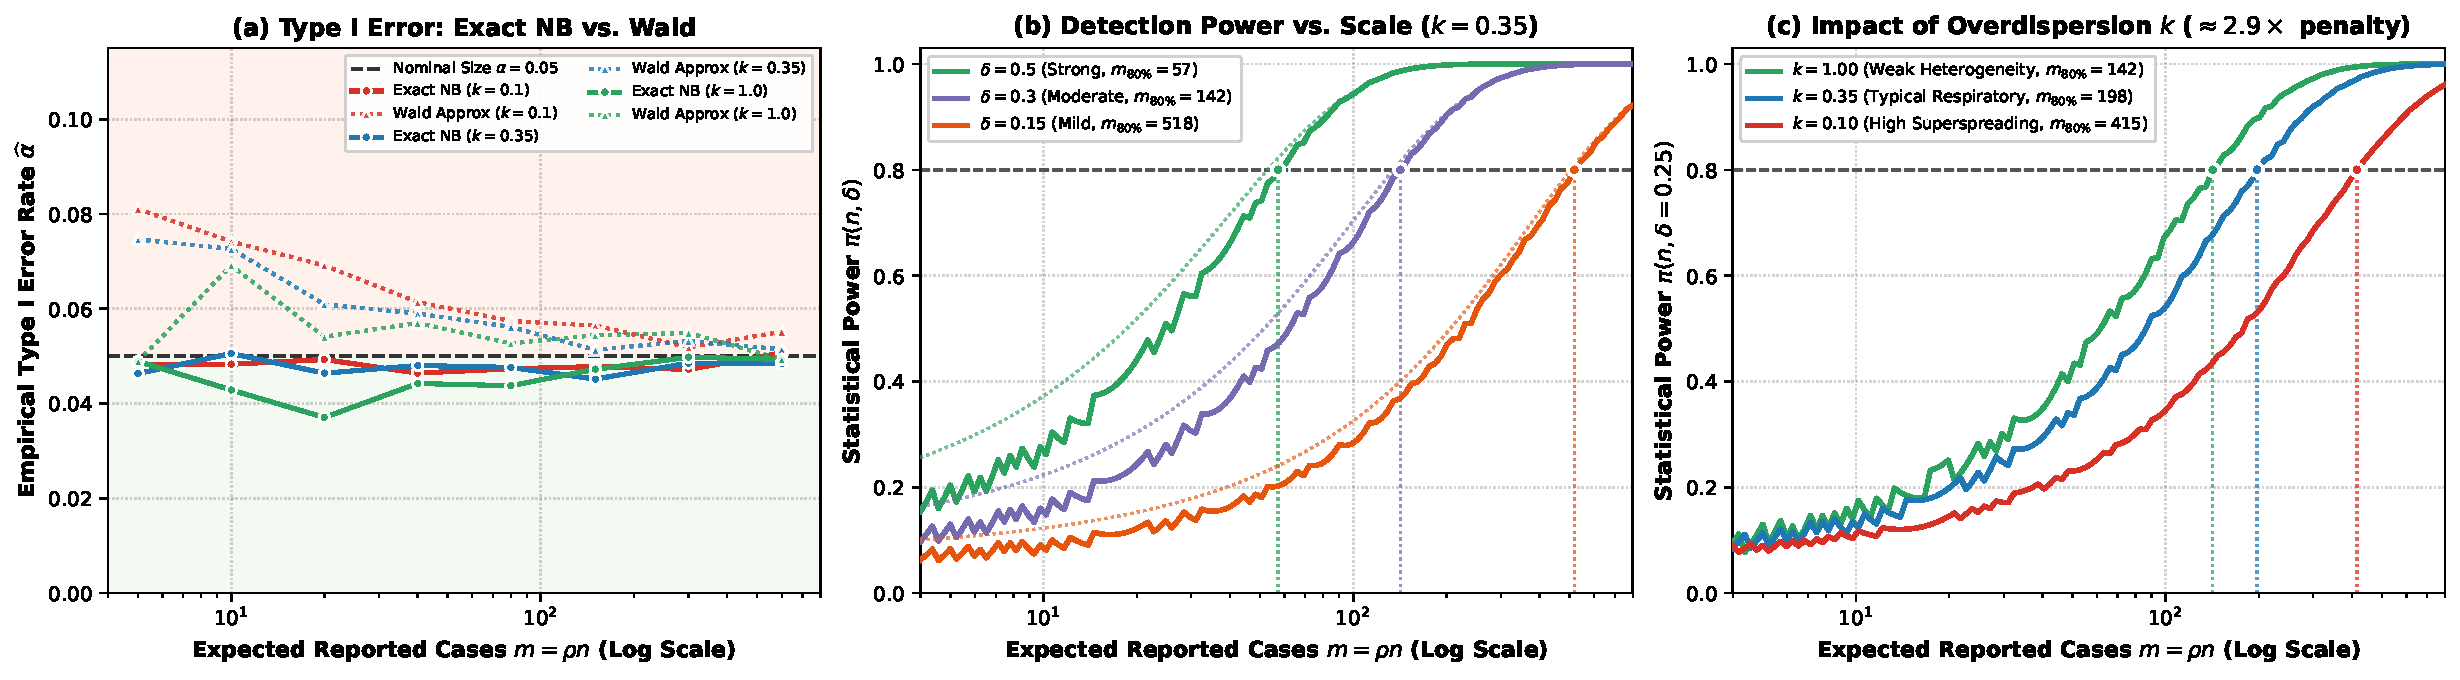
\includegraphics[width=0.92\textwidth]{figures/fig2_growth_detection_power.pdf}
\caption{\textbf{早期暴发检验尺度效应、功效边界与超传播惩罚。}
(a) 一类错误率控制：渐近正态 Wald 检验（虚线）在低病例规模（$m < 40$）且严重超传播（$k=0.1$）时经验一类错误率最高达 8.1\%（$m=5$），系统性高于名义水平 0.05（严重虚警）；离散精确负二项检验（实线）在全样本网格上严格控制错误率低于 0.05。(b) 检出功效曲线随备择强度 $\delta = R_t - 1$ 的响应：在 $k=0.35$ 时，达到 80\% 功效所需的期望报告规模由微弱暴发 $\delta=0.15$ 的 $m=517.8$ 急剧下降至 $\delta=0.30$ 的 $m=142.0$ 与 $\delta=0.50$ 的 $m=57.2$。(c) 个体超传播离散度 $k$ 的杠杆惩罚：在 $\delta=0.25$ 增长强度下，达到 80\% 检出功效所需的期望病例数从低异质性 $k=1.0$ 的 $m=142.0$ 急剧上升至严重超传播 $k=0.1$ 的 $m=415.0$，规模需求放大了近 3 倍。标称显著性水平 $\alpha = 0.05$，基准报告率 $\rho = 0.25$。}
\label{fig:detection_power}
\end{figure}

数值模拟揭示出两项极为关键的结论：
\begin{enumerate}[label=(\arabic*)]
    \item **经典渐近正态 Wald 检验在小规模段严重失真**：
    传统软件（如经典 t 检验或 Wald 检验）在小病例数且高离散时，假定统计量渐近正态，导致经验一类错误率最高达到 8.1\%，严重超出 5\% 的名义红线，频繁发出疫情失控的假警报；而基于命题 5 构建的精确离散负二项检验在全参数网格上严格受控于 0.05 以下；
    \item **检验目标存在天然饱和天花板**：
    与单代点估计无界降方差不同，一旦样本规模越过充分检出阈值 $m_{80\%}$，统计功效迅速逼近 1.0 平台。继续扩大监测网络已无法产生任何实质性的预警增益。
\end{enumerate}

\section{命题 6：更新过程条件预测误差全方差分解}\label{sec:prop6_renewal}

本节将推断推进至时间序列更新过程动态预测场景。在真实监测中，下一代新发病例是通过历史报告病例的滑动卷积进行预测的，此过程不仅包含单代抽样方差，更包含了状态代理偏差。

\subsection{两步全方差公式展开与式 (29) 偏差项推导}

\begin{proposition}[\textbf{命题 6：更新过程单步预测误差条件全方差分解}]\label{prop:prop6}
基于截至第 $t$ 期的报告信息集 $\mathcal{F}_t^C$：
\begin{enumerate}[label=(\roman*)]
    \item 未来真实感染数 $I_{t+1}$ 的预测方差严格满足全方差恒等式：
    \begin{equation}
    \Var(I_{t+1} \mid \mathcal{F}_t^C) = \Var\big( \Lambda_{t+1} R_{t+1} \;\big|\; \mathcal{F}_t^C \big) + \E\Big[ \Var\big( I_{t+1} \;\big|\; \Lambda_{t+1}, R_{t+1}, \mathcal{F}_t^C \big) \;\Big|\; \mathcal{F}_t^C \Big]; \label{eq:var_I_decomp}
    \end{equation}
    \item 未来报告病例数 $C_{t+1}$ 的观测预测方差满足：
    \begin{equation}
    \Var(C_{t+1} \mid \mathcal{F}_t^C) = \rho(1 - \rho)\,\E[I_{t+1} \mid \mathcal{F}_t^C] + \rho^2 \Var(I_{t+1} \mid \mathcal{F}_t^C); \label{eq:var_C_decomp}
    \end{equation}
    \item 记事后代理增长比为 $G_{t+1} \triangleq C_{t+1} / D_t$，其中 $D_t \triangleq \sum_{s=1}^p w_s C_{t+1-s}$ 为历史加权有效暴露规模。设 $\mu_{t+1 \mid t} \triangleq \E[C_{t+1} \mid \mathcal{F}_t^C]$ 与 $\sigma_{t+1 \mid t}^2 \triangleq \Var(C_{t+1} \mid \mathcal{F}_t^C)$，在活跃周（$D_t > 0$）上有严格的条件预测均方误差正交分解（式 29 / 式 380）：
    \begin{equation}
    \E\left[ (G_{t+1} - \bar{R})^2 \;\middle|\; D_t > 0 \right] = \E\left[ \frac{\sigma_{t+1 \mid t}^2}{D_t^2} + \left( \frac{\mu_{t+1 \mid t}}{D_t} - \bar{R} \right)^2 \;\middle|\; D_t > 0 \right]. \label{eq:exact_renewal_decomp}
    \end{equation}
\end{enumerate}
\end{proposition}

\begin{proof}
证明分两步应用全方差公式：

\textbf{第一步：潜在真实感染 $I_{t+1}$ 预测方差分解}
在更新过程假设下，给定历史传播压力 $\Lambda_{t+1}$ 与当期环境 $R_{t+1}$，真实感染期望为 $\Lambda_{t+1} R_{t+1}$。直接以历史信息及当期传播压力 $(\Lambda_{t+1}, R_{t+1})$ 为条件应用全方差公式，即得式~\eqref{eq:var_I_decomp}。

\textbf{第二步：报告病例数 $C_{t+1}$ 预测方差分解}
以未观测的潜在真实感染 $I_{t+1}$ 为条件再次应用全方差公式：
\begin{equation}
\Var(C_{t+1} \mid \mathcal{F}_t^C) = \E\big[ \Var(C_{t+1} \mid I_{t+1}, \mathcal{F}_t^C) \;\big|\; \mathcal{F}_t^C \big] + \Var\big( \E[C_{t+1} \mid I_{t+1}, \mathcal{F}_t^C] \;\big|\; \mathcal{F}_t^C \big).
\end{equation}
由条件二项报告抽样假定 $C_{t+1} \mid (I_{t+1}, \mathcal{F}_t^C) \sim \Binomial(I_{t+1}, \rho)$，有条件方差 $\Var(C_{t+1} \mid I_{t+1}, \mathcal{F}_t^C) = I_{t+1}\rho(1-\rho)$ 与条件均值 $\E[C_{t+1} \mid I_{t+1}, \mathcal{F}_t^C] = \rho I_{t+1}$。代入得：
\begin{equation}
\Var(C_{t+1} \mid \mathcal{F}_t^C) = \E\big[ I_{t+1}\rho(1-\rho) \;\big|\; \mathcal{F}_t^C \big] + \Var\big( \rho I_{t+1} \;\big|\; \mathcal{F}_t^C \big) = \rho(1-\rho)\E[I_{t+1} \mid \mathcal{F}_t^C] + \rho^2 \Var(I_{t+1} \mid \mathcal{F}_t^C).
\end{equation}
式~\eqref{eq:var_C_decomp} 证毕。

\textbf{第三步：式~\eqref{eq:exact_renewal_decomp} 均方误差正交展开}
由条件期望的加减项配方恒等式：
\begin{align}
\E\left[ (G_{t+1} - \bar{R})^2 \;\middle|\; \mathcal{F}_t^C \right] &= \E\left[ \left( \frac{C_{t+1}}{D_t} - \frac{\mu_{t+1 \mid t}}{D_t} + \frac{\mu_{t+1 \mid t}}{D_t} - \bar{R} \right)^2 \;\middle|\; \mathcal{F}_t^C \right] \notag \\
&= \E\left[ \left( \frac{C_{t+1} - \mu_{t+1 \mid t}}{D_t} \right)^2 \;\middle|\; \mathcal{F}_t^C \right] + \left( \frac{\mu_{t+1 \mid t}}{D_t} - \bar{R} \right)^2 \notag \\
&\quad + 2 \left( \frac{\mu_{t+1 \mid t}}{D_t} - \bar{R} \right) \cdot \frac{\E[C_{t+1} - \mu_{t+1 \mid t} \mid \mathcal{F}_t^C]}{D_t}.
\end{align}
由条件期望定义，交叉项 $\E[C_{t+1} - \mu_{t+1 \mid t} \mid \mathcal{F}_t^C] \equiv 0$ 严格恒等于零！因此：
\begin{equation}
\E\left[ (G_{t+1} - \bar{R})^2 \;\middle|\; \mathcal{F}_t^C \right] = \frac{\sigma_{t+1 \mid t}^2}{D_t^2} + \left( \frac{\mu_{t+1 \mid t}}{D_t} - \bar{R} \right)^2.
\end{equation}
对信息集 $\mathcal{F}_t^C$（在 $D_t > 0$ 支撑集上）取全期望，即得式~\eqref{eq:exact_renewal_decomp}。命题 6 证毕。
\end{proof}

\subsection{更新过程双口径争议彻底澄清}
式~\eqref{eq:exact_renewal_decomp} 清晰揭示了更新过程较之单代静态基准所增加的两个关键机制：
\begin{enumerate}[label=(\alph*)]
    \item 随机分母 $D_t$ 对条件方差的倒数二次方重新加权；
    \item 用报告历史代理真实感染压力导致的**非负预测偏差项** $\left(\frac{\mu_{t+1 \mid t}}{D_t} - \bar{R}\right)^2 \ge 0$。
\end{enumerate}

\begin{figure}[htbp]
\centering
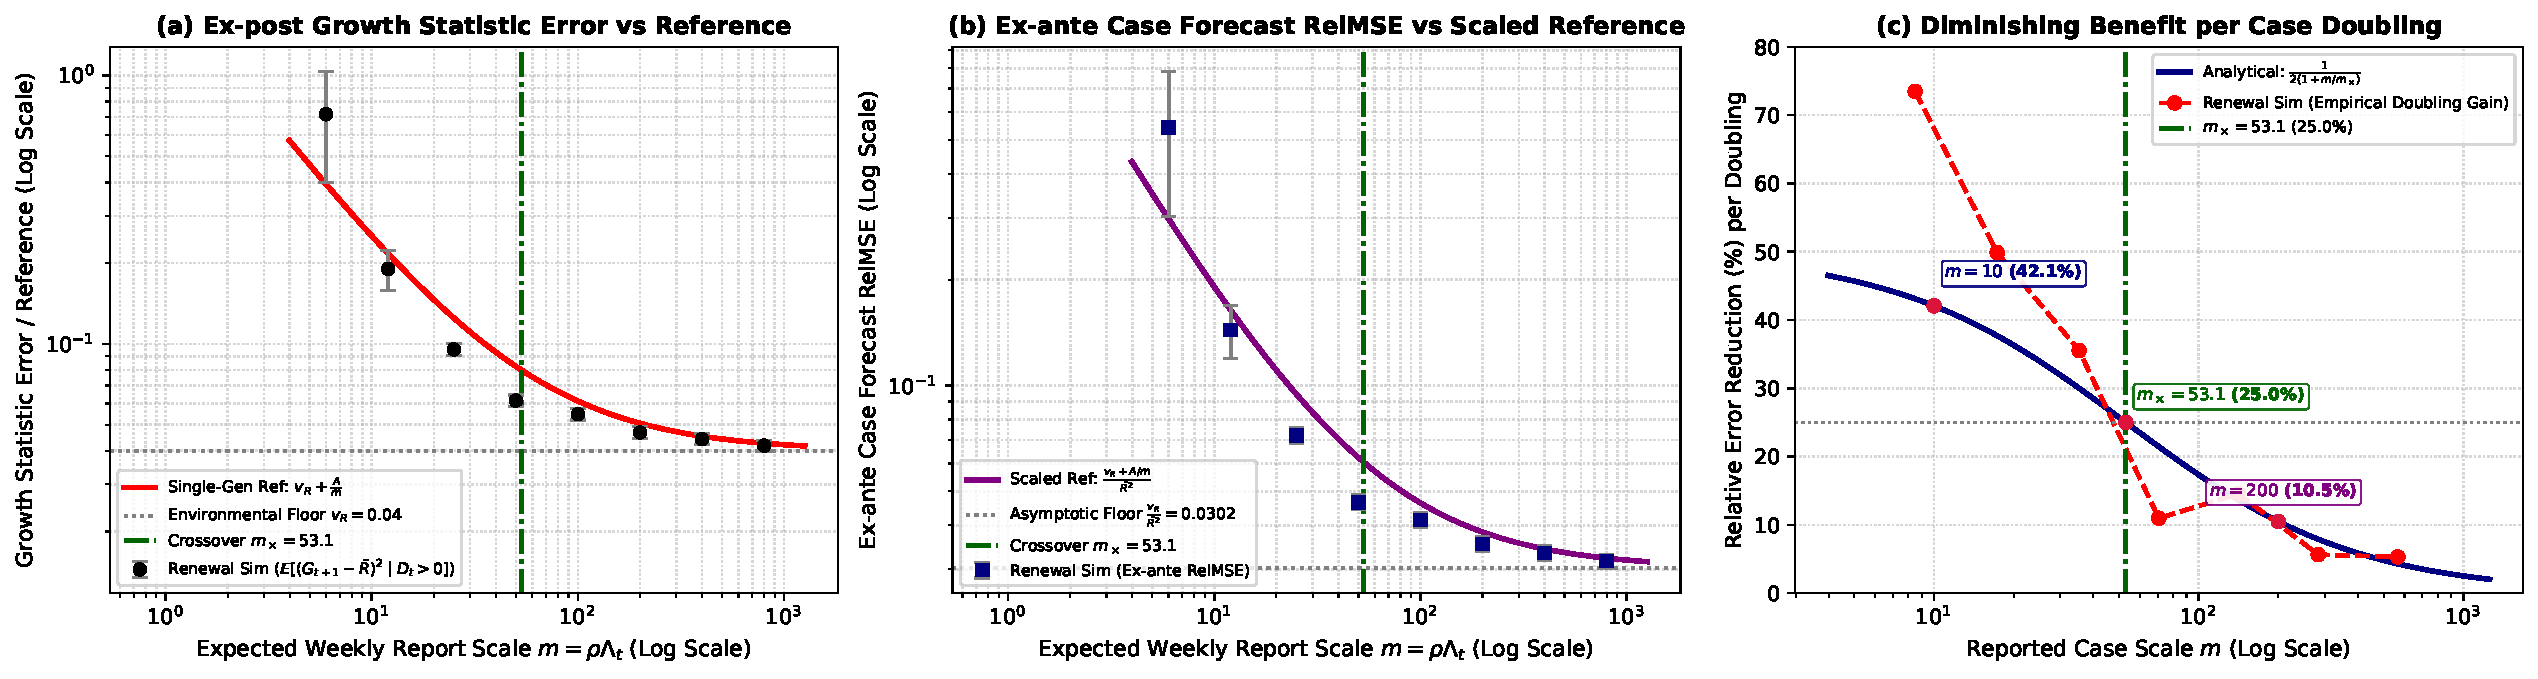
\includegraphics[width=0.92\textwidth]{figures/fig3_forecasting_saturation_crossover.pdf}
\caption{\textbf{更新过程时序卷积下事后增长统计量与事前单步病例预测误差。}
(a) 事后代理增长统计量随规模衰减轨迹，在中大规模段贴合单代参照 $v_R + A/m$，在小规模段被随机分母二次放大。(b) 事前病例预测相对均方误差（RelMSE）与参照曲线对比。(c) 边际削减收益定量衰减规律：规模翻倍的方差下降比例严格由式~\eqref{eq:variance_halving} 给出，越过平衡点后急剧放缓。}
\label{fig:forecasting_crossover}
\end{figure}

图~\ref{fig:forecasting_crossover} 展现了更新过程模拟的关键现象，并彻底厘清了所谓的“口径张力”：
\begin{itemize}
    \item **初始参数口径（0.75--0.98 倍）**：若横轴按第 0 周的初始生成参数 $m$ 排列，由于模拟设定 $\bar{R} = 1.15 > 1$（疫情处于自发指数增长态势），到了第 4--29 周评价时，实际周病例规模中位数已达初始值的 1.7--2.4 倍（均值口径约为 2.6--3.2 倍）。拿增长后的大病例数去对比初始小规模的理论值，表观比值显得低于参照线；
    \item **实际实现规模分箱口径（1.01--1.17 倍，按组 1.00--1.45 倍）**：若按评价周实际发生的病例暴露规模重核参照线，更新过程经验预测误差**始终严格不低于单代静态下界**！这在数值上直接证实了式~\eqref{eq:exact_renewal_decomp} 所预言的额外非负预测偏差项。
\end{itemize}

针对解析参照曲线 $V(m) = v_R + A/m$，病例规模翻倍时的相对方差下降比例严格满足：
\begin{equation}
\frac{V(m) - V(2m)}{V(m)} = \frac{\left( v_R + \frac{A}{m} \right) - \left( v_R + \frac{A}{2m} \right)}{v_R + \frac{A}{m}} = \frac{\frac{A}{2m}}{v_R + \frac{A}{m}} = \frac{1}{2\left( 1 + \frac{m}{m_\times} \right)}. \label{eq:variance_halving}
\end{equation}
当 $m = 10$ 时，规模翻倍可降低约 42.1\% 的解析方差；越过交叉点 $m_\times \approx 53.1$ 后，当 $m = 200$ 时，病例规模再翻倍仅能带来约 10.5\% 的方差削减。这印证了本文的核心定性直觉：**越过平衡点后，单纯扩大捕获规模的边际改善速率急剧放缓**。
